% !TeX root = ../main.tex
\chapter{绪论}

\section{研究的背景和意义}


数据中心是互联网的 ``大脑'',也是人类存储海量数据、进行大规模计算和提供互联网服务的基础设施。21 世纪第一个十年,数据中心主要处理 Web 网站、搜索引擎等容易并行的任务;通用处理器的高速性能提升也使得专用硬件的优势不甚明显。因此,互联网数据中心多使用大量低成本的标准服务器搭建。

近十年来,大数据与人工智能的兴起改变了数据中心的应用负载特性。一方面,大数据处理、机器学习等负载对算力要求很高。然而,由于摩尔定律的放缓和 Dennard 缩放定律的终结,近十年来,通用处理器的频率提升和多核核数增加都受到功耗墙的限制。因此,通用处理器性能提升 ``免费的午餐'' 已经结束,体系结构的创新迎来了春天,GPU、FPGA、TPU 等定制化硬件在数据中心内大量部署。另一方面,大数据处理、机器学习等负载需要多个节点紧密协同处理,对节点间的通信带宽和延迟要求较高。因此,近十年来,数据中心网络从 1 Gbps 发展到 40 Gbps,并有向 100 Gbps 演进的趋势。定制化硬件之间的专用互连也成为趋势。因此,如英伟达 CEO 黄仁勋所说,未来的数据中心会像超级计算机一样 \cite{nvidia-datacenter}。

与此同时,数据中心的运营模式也在经历一场云化的变革。数据中心的算力逐渐集中到少数几家云厂商,每家拥有数以百万计的服务器。由于云数据中心的规模大,云服务商有足够的规模来平摊服务器、板卡甚至芯片的设计和流片成本,通过软件优化也可以提高性能指标、降低成本,获得可观的经济效益。由于上述应用负载特性的转变和数据中心的云化,工程师获得了从硬件、系统软件到应用的全栈优化机会。

在云数据中心中,不同的租户共享一个巨大的计算、存储和网络资源池。为了实现资源共享和性能隔离,数据中心需要实现计算、存储和网络的虚拟化。如图 \ref{intro:fig:virt-architecture} 所示,在基础设施作为服务(IaaS)的云服务模式下,计算节点上需要提供虚拟网络、虚拟云存储、虚拟本地存储等服务,实际的网络和云存储资源则位于独立的网络节点和存储节点上。计算节点上的虚拟网络和存储服务把数据中心内物理上分散的网络和存储资源虚拟化成逻辑上统一的资源(``多虚一'')。网络和存储节点则不仅需要把物理资源共享给多个计算节点上不同租户的虚拟机使用(``一虚多''),还需要提供数据处理功能和高层抽象。网络节点需要提供防火墙、负载均衡、加密隧道网关、网络地址转换(NAT)等网络功能;存储节点需要进行数据结构处理以提供对象存储、文件系统存储等高层抽象,还需要进行复制(replication)以实现容灾。


\begin{figure}[htbp]
	\centering
	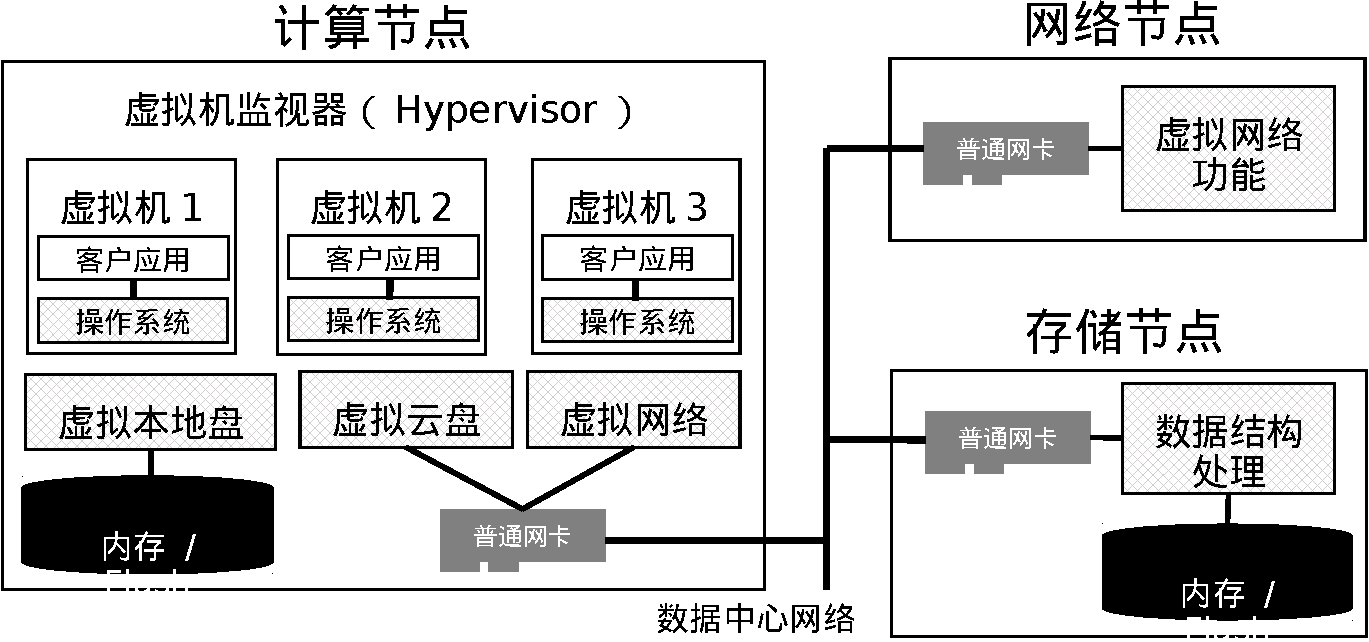
\includegraphics[width=0.8\textwidth]{figures/virt_arch.pdf}
	\caption{虚拟化的数据中心架构。}
	\label{intro:fig:virt-architecture}
\end{figure}


由于云服务的快速迭代,这些虚拟化的网络、存储功能还需要灵活性、可编程性和可调试性,传统上往往用运行在通用处理器上的软件实现。除了虚拟化开销,传统操作系统的开销也不容忽视。这些图 \ref{intro:fig:virt-architecture} 中蓝色方框所示的软件开销被称为 ``数据中心税''(data center tax) \cite{barroso2009datacenter,barroso2013datacenter,barroso2017attack,barroso2018datacenter}。
在网络、存储、定制化计算硬件越来越快的趋势下,数据中心税不仅浪费了大量的 CPU 资源,还导致应用程序无法充分利用硬件的性能。
例如,我们将在第 \ref{chapter:clicknp} 章看到,计算节点需要占用 20\% 左右的 CPU 用来实现网络和存储虚拟化,而计算节点的虚拟网络和网络节点的网络功能都会增加数十乃至上千微秒的延迟。作为比较,数据中心网络本身的延迟只有数微秒至数十微秒,虚拟化增加的延迟比网络本身的延迟还高。
我们也将在第 \ref{chapter:kvdirect} 章看到,软件数据结构存储的性能不仅与内存性能相去甚远,甚至连充分利用持久化闪存的性能都困难。
我们还将在第 \ref{chapter:socksdirect} 章看到,应用程序普遍使用操作系统中的套接字原语来进行通信,对于 Web 服务器等通信密集型的应用程序,操作系统占用了 50\% 至 90\% 的 CPU 时间;而且,操作系统实现的套接字原语比硬件提供的远程直接内存访问(RDMA)原语延迟高一个数量级。

综上,通过软硬件结合的全栈优化降低 ``数据中心税'' 对现代数据中心的性能和成本有重要意义,这也是本文研究的课题。





\section{国内外研究现状}


随着通用处理器的性能提升遇到了瓶颈,各大云服务商开始探索使用定制化硬件来 ``减税降负'',也就是把数据中心的虚拟化、操作系统和高层抽象的开销从通用处理器转移到定制化硬件上。
本质上,这与 GPU 等定制化计算硬件的加速原理类似,即用硬件实现规则的、通用的操作,而把不规则的、不常用的操作留给通用处理器上的软件。

在数据中心税中,由于大规模 Web 服务、大数据处理、机器学习等应用对网络的性能需求非常迫切,软件虚拟网络又很难以可接受的成本提供如此高的性能,可编程网卡是最早被公有云大规模部署的定制化硬件之一。
以微软 Azure 云为代表的云服务商在数据中心的每台服务器上部署了一块可编程网卡,用以加速计算节点上的虚拟网络 \cite{smartnic}。
为了在提供高性能的同时保持一定的可编程性和灵活性,业界提出了专用芯片(ASIC)、网络处理器(Network Processor)、多核通用处理器片上系统(SoC)、现场可编程门阵列(FPGA)等可编程网卡架构。





学术界网络功能虚拟化(NFV)软件(NetBricks 等),GPU 等……

学术界还提出了用柜顶网络交换机(Top-of-Rack switch)和图形处理器(GPU)加速网络功能。

学术界也提出了多种基于专用芯片的可编程网卡架构……
基于专用芯片的柜顶交换机和可编程网卡灵活性较差,而基于通用处理器的可编程网卡和 GPU 有一定的性能局限性。
FPGA 在性能和灵活性间达到了折中,因此微软采用了基于 FPGA 的可编程网卡 \cite{putnam2014reconfigurable}。

FPGA 编程,SoC 可编程网卡编程……

AWS …… 国内 ……

除了网络系统,本文进一步探索存储系统和操作系统的优化。


加州大学伯克利分校对无服务器计算(serverless computing)的预测报告 \cite{jonas2019cloud} 表明,尽管无服务器计算的范式有诸多优势,也是各大云服务商争相推广的新服务,但由于云存储的性能问题和临时存储服务的缺失,很多类型的应用使用无服务器计算的性能和成本不理想。

RDMA 数据结构、数据库事务、存储虚拟化……

网络协议栈加速,软件加速方案(eRPC 等)……



\section{本文的研究内容和贡献}


本文旨在探索基于可编程网卡的高性能数据中心系统。本文提出一个基于 FPGA 可编程网卡,对云计算数据中心计算、网络、存储节点实现全栈加速的系统。如图 \ref{arch:fig:accel-arch} 所示……


\begin{figure}[htbp]
	\centering
	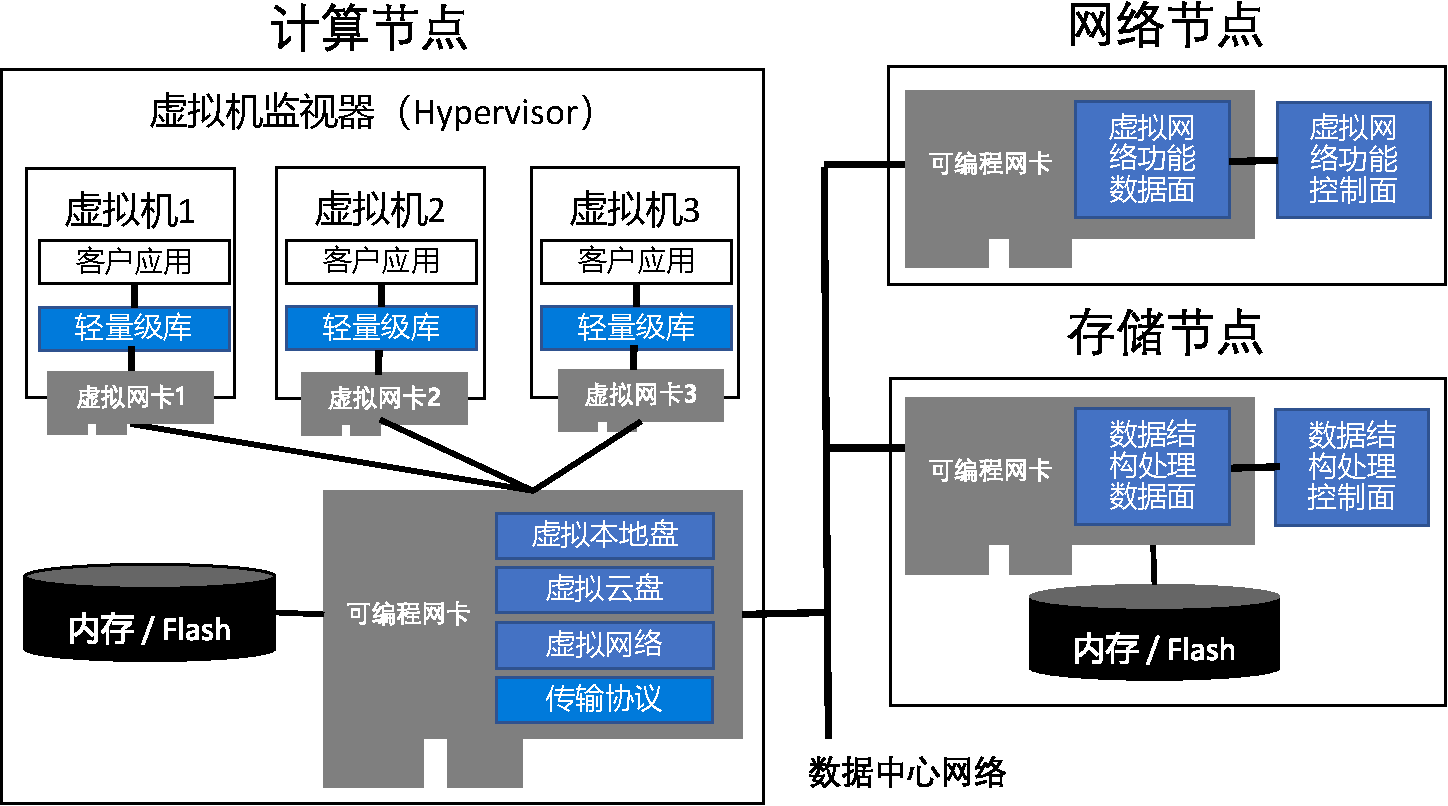
\includegraphics[width=0.8\textwidth]{figures/accel_arch.pdf}
	\caption{基于可编程网卡的数据中心系统总体架构。}
	\label{arch:fig:accel-arch}
\end{figure}

首先,本文提出用可编程网卡加速云计算中的虚拟网络功能。我们提出了首个在商用服务器中用 FPGA 加速的高灵活性、高性能网络功能处理平台 ClickNP。众所周知,FPGA 编程对软件工程师很不友好。为了简化 FPGA 编程,我们设计了类 C 的 ClickNP 语言和模块化的编程模型,并开发了一系列优化技术,以充分利用 FPGA 的海量并行性。我们实现了 ClickNP 开发工具链,可以与多种商用高层次综合工具集成。我们基于 ClickNP 设计和实现了 200 多个网络元件,并用这些元件组建起多种网络功能。相比基于 CPU 的软件网络功能,ClickNP 的吞吐量提高了 10 倍,延迟降低到 1/10;且具有可忽略的 CPU 开销,可以为云计算中的每个计算节点节约 20\% 的 CPU 核。

其次,本文提出用可编程网卡加速远程数据结构访问。键值存储是最常用的基本数据结构之一,也是很多数据中心内的关键分布式系统组件。我们基于 ClickNP 编程框架,设计实现了一个高性能内存键值存储系统 KV-Direct,在服务器端绕过 CPU,用可编程网卡通过 PCIe 直接访问主机内存。我们把单边 RDMA 的内存操作语义扩展到键值操作语义,解决了单边 RDMA 操作数据结构时通信和同步开销高的问题。我们还利用 FPGA 可重配置的特性,允许用户实现更复杂的数据结构。面对网卡与主机内存之间 PCIe 带宽较低、延迟较高的性能挑战,我们设计了哈希表、内存分配器、乱序执行引擎、负载均衡和缓存、向量操作等一系列性能优化,实现了 10 倍于 CPU 的能耗效率和微秒级的延迟,实现了首个单机性能达到 10 亿次每秒的通用键值存储系统。

最后,本文提出用可编程网卡和用户态运行库相结合的方法为应用程序提供系统原语,从而绕过操作系统内核。套接字是操作系统提供的最常用的通信原语。我们设计实现了一个用户态套接字系统 SocksDirect,与现有应用程序完全兼容,能实现接近硬件极限的吞吐量和延迟,多核性能具有可扩放性,并在高并发负载下保持高性能。我们分别使用共享内存和 RDMA 实现主机内和主机间的通信。为了支持高并发连接数,我们基于 KV-Direct 实现了一个 RDMA 可编程网卡。我们消除了线程间同步、缓冲区管理、大数据拷贝、进程唤醒等一系列开销。SocksDirect 相比 Linux 提升了 7 至 20 倍吞吐量,降低延迟到 1/17 至 1/35,并将 Web 服务器的 HTTP 延迟降低到 1/5.5。


\section{论文结构安排}

本论文的内容结构安排如下:
第 1 章为绪论。
第 2 章介绍了数据中心的背景知识和硬件的发展趋势,分析了可编程网卡的四种架构,并调研了可编程网卡在数据中心的应用。
第 3 章提出了基于可编程网卡的高性能数据中心系统架构。
第 4 章提出用可编程网卡加速云计算中的虚拟网络功能。为了简化FPGA编程,提出了首个适用于高速网络数据包处理、基于高级语言的模块化FPGA编程框架ClickNP。
第 5 章提出用可编程网卡加速远程数据结构访问,并设计实现了一个高性能内存键值存储系统 KV-Direct。
第 6 章提出用可编程网卡和用户态运行库相结合的方法为应用程序提供操作系统原语,并设计实现了一个用户态套接字系统 SocksDirect。
第 7 章总结全文并展望未来研究方向。